\item \points{2d} {\bf Experiments - Adjusting Learning Rate and Inner Loop Steps}

\begin{enumerate}[label=(\roman*)]
    \item Try MAML with the same hyperparameters as above except for a fixed inner learning rate of $0.04$ by running \texttt{python maml.py --inner\_lr 0.04}

    Your plot of the validation post-adaptation query accuracy over the course of training with the two inner learning rates ($0.04$, $0.4$) should look as follows.
    \begin{center}
        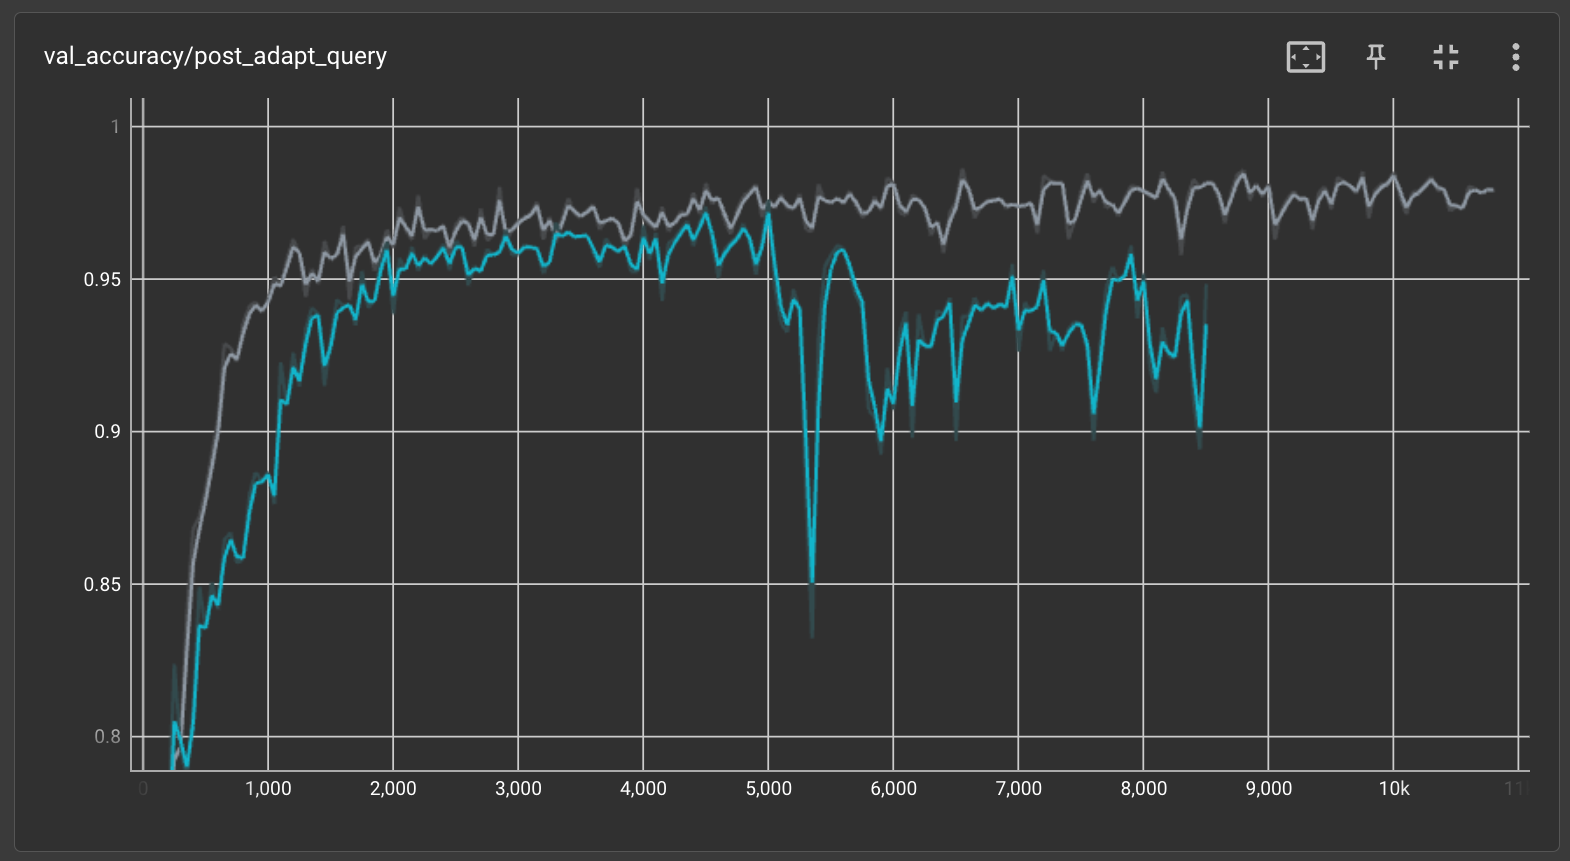
\includegraphics[width=0.75\linewidth]{./figures/maml_q3}
    \end{center}
    
    What is the effect of lowering the inner learning rate on (outer-loop) optimization and generalization?

    \item Try MAML with a fixed inner learning rate of $0.04$ for $5$ inner loop steps by \texttt{python maml.py --inner\_lr 0.04 ----num\_inner\_steps 5}

    Your plot of the validation post-adaptation query accuracy over the course of training with the two number of inner loop steps ($1$, $5$) with inner learning rate $0.04$ should look as follows.
    \begin{center}
        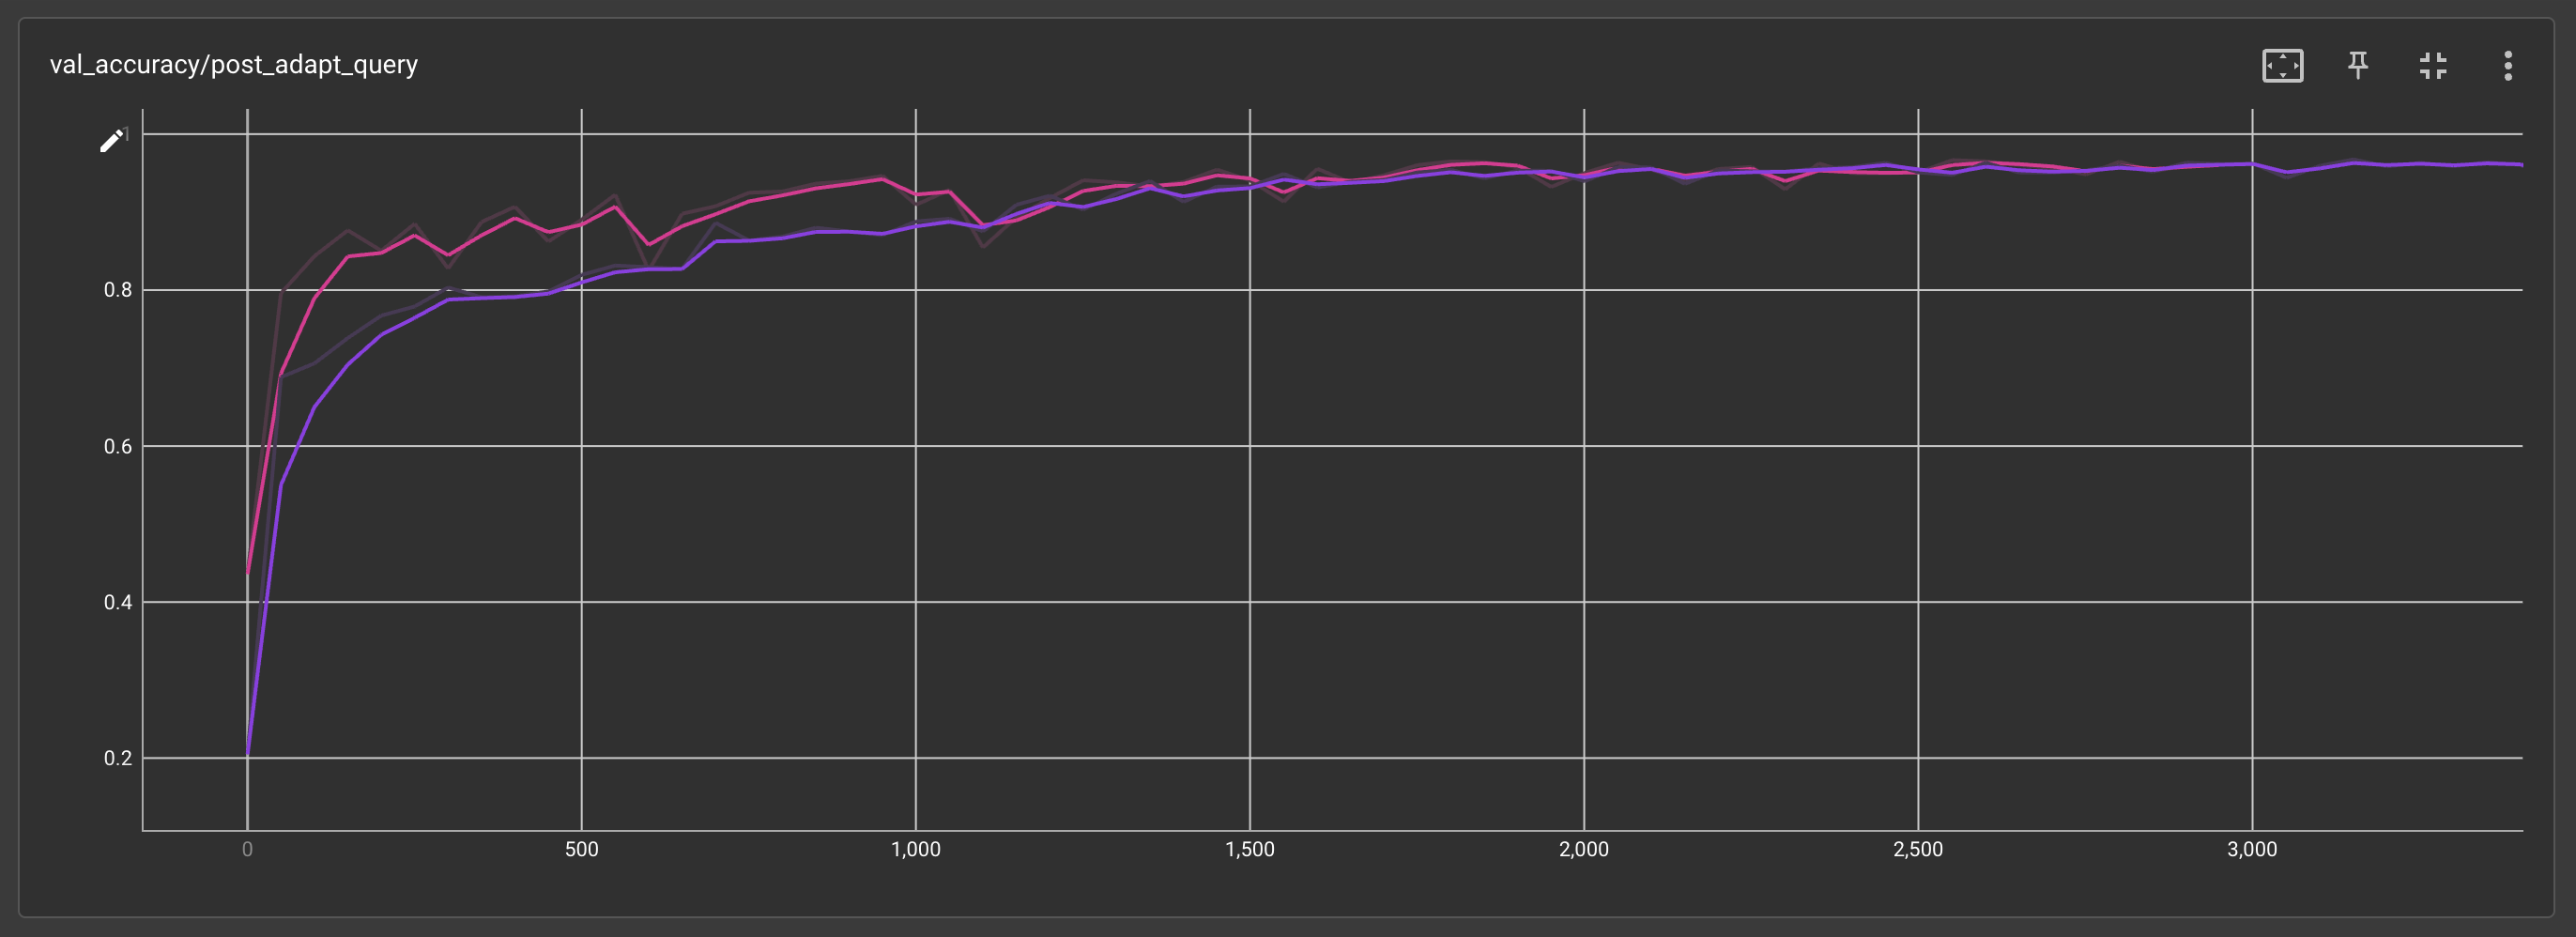
\includegraphics[width=0.75\linewidth]{./figures/maml_q4}
    \end{center}

    What is the effect of increasing the number of inner loop steps on (outer-loop) optimization and generalization?

    \item Try MAML with learning the inner learning rates by running \texttt{python maml.py --learn\_inner\_lrs}. Initialize the inner learning rates with $0.4$.

    Your plot of the validation post-adaptation query accuracy over the course of training for learning and not learning the inner learning rates, initialized at $0.4$ should look as follows.
    \begin{center}
        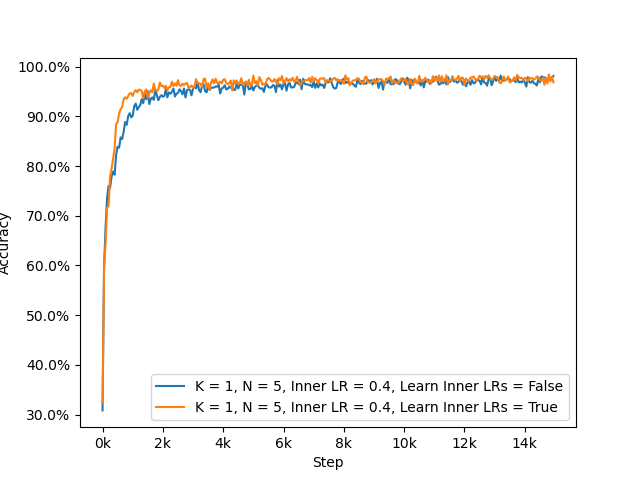
\includegraphics[width=0.75\linewidth]{./figures/maml_q5}
    \end{center}

    What is the effect of learning the inner learning rates on (outer-loop) optimization and generalization?
\end{enumerate}